\section{Decomposing the Wall Clock}
\label{sec:model}

\subsection{Two components}

We split the wall clock at every sampled instant according to whether the
engine has any request in flight:
\begin{equation}
  W \;=\; W_{\text{busy}} \;+\; W_{\text{idle}} .
  \label{eq:split}
\end{equation}
Fig.~\ref{fig:decomp} shows the split for every completed run. Two things are
immediately visible and both matter later.

First, idle time is not noise. It ranges from 7.4\% of the wall clock for the
fastest configuration to 36.3\% for the slowest. The individual stretches are
long---median 10--20\,s, p90 20--60\,s, maximum 511\,s over 1{,}849 stretches
(Fig.~\ref{fig:idle})---which places them at the same scale as the mean tool
wait of 16.85\,s. This is not a sampling artifact: we sampled every 5\,s over
runs of 3--9 hours, so 10\,s is the smallest resolvable stretch.

Second, the two components move independently. \texttt{bres}
(\S\ref{sec:results}) reduces idle from 15.9\% to 10.1\%, recovering about 17
minutes---and is nonetheless \emph{slower} than its own baseline, because its
busy time grows by 21 minutes. Any account that treats ``more concurrency'' as
one thing will get this wrong.

\begin{figure}[tb]
  \centering
  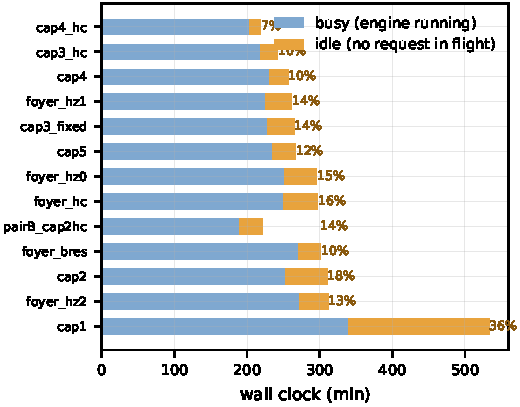
\includegraphics[width=\columnwidth]{figs/fig2_decomp.pdf}
  \caption{Wall clock split into busy and idle for every completed run,
  ordered by total duration. Idle is 7.4\% for the fastest configuration and
  36.3\% for the slowest. Note \texttt{bres}: it cuts idle to 10.1\% and is
  still slower than its own baseline, because busy time grows instead.}
  \label{fig:decomp}
\end{figure}

\subsection{What determines busy time}

During busy time the engine executes steps; each step produces one token per
running request. Hence
\begin{equation}
  W_{\text{busy}} \;\approx\; \frac{G}{\overline{R}}\,\tau ,
  \label{eq:busy}
\end{equation}
with $G$ the total generated tokens (fixed by the trace at 706{,}010) and
$\tau$ the per-step cost. Across our runs $\tau$ is not a fit parameter we
tuned; we obtain it two ways and check that they agree.

\paragraph{Method 1 (derived).} $\tau_1 = W_{\text{busy}} \cdot \overline{R} /
G$, using the engine's own \texttt{num\_running\_reqs} for $\overline{R}$. The
time term must be the busy component and not the wall clock: using the wall
clock charges a run's idle time to its steps, which inflates $\tau_1$ by
$1/(1-\text{idle fraction})$---38\% for \texttt{cap1} at 36.3\% idle, against
a per-request measurement that differs from ours by 11\%. With the busy
component the two methods agree to within 12\% on every run.

\paragraph{Method 2 (independent).} For each step record we compute the
per-request decode interval,
$(\text{total\_duration} - \text{first\_token}) / (\text{output\_len} - 1)$,
and take the median over steps with $\text{output\_len} \ge 32$.

The two agree to within 12\% on every run---Method 1 includes prefill that
Method 2 excludes---and they rank the runs nearly identically (Spearman
$\rho = 0.967$; the residual disagreements are all adjacent swaps between runs
whose step times differ by under 2\,ms, Fig.~\ref{fig:steptime}). This matters
because Method 1 alone would be circular: it derives $\tau$ from the quantity
it is used to explain. Method 2 does not, and it recovers the same structure.
We state the strength of this claim precisely: we have two consistent derived
measurements of step time, not an engine-reported one. The engine's own latency counters
(\texttt{itl\_p50}, \texttt{e2e\_p50}, \texttt{ttft\_p50}) are exported as zero
by SGLang v0.5.10 in our configuration, so no directly measured step time
exists in our data; instrumenting this is future work.

\begin{figure}[tb]
  \centering
  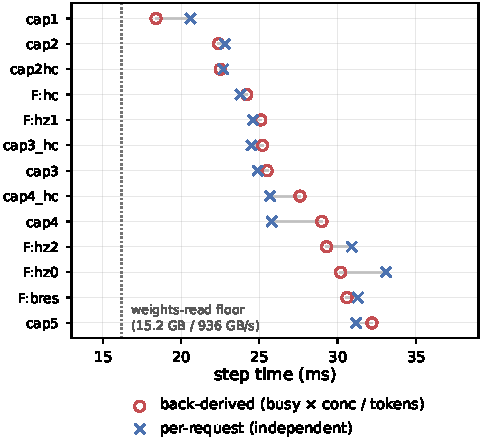
\includegraphics[width=\columnwidth]{figs/fig3_steptime.pdf}
  \caption{Per-step cost by two independent measurements, one run per row:
  circles derive it from busy time, crosses from per-request decode intervals.
  They agree to within 12\% and rank the runs nearly identically
  ($\rho = 0.967$). The dotted line is the cost of reading the weights once;
  every run sits above it.}
  \label{fig:steptime}
\end{figure}

\subsection{The per-step cost is not constant in concurrency}

Equation~\ref{eq:busy} would be uninteresting if $\tau$ were a constant. It is
not. Across our 13 runs $\tau$ ranges from 18.4 to 32.2\,ms (Method 1) and
20.6 to 33.1\,ms (Method 2), and it correlates with the running count:
$r = 0.85$ by Method 1, $r = 0.62$ by Method 2.

The correlation is loose, and the looseness is itself the finding. The two
configurations with the highest running counts behave differently:
\texttt{cap4\_hc} runs 1.60 requests at 27.6\,ms while \texttt{F:hz0} runs
1.41 at 30.2\,ms. Running count sets a floor and a trend, not a value.

This is still the crux of the paper, because the arithmetic of
Eq.~\ref{eq:busy} is unforgiving. Take $\tau$ at its low end, 18.4\,ms, and
\texttt{cap5}'s busy time would be 134 minutes instead of the measured 234.
The rise in $\tau$ absorbs 100 minutes---more than half of what raising
$\overline{R}$ from 0.64 to 1.62 buys. An admission policy can raise
$\overline{R}$; it cannot raise it without raising $\tau$; and the second
effect eats the first.

\paragraph{A mechanism we proposed and had to withdraw.} Our first account was
that a full pool forces evictions, and that an evicted prefix must be
recomputed when its session returns, with that recomputation chunked into
decode steps. Two direct counters refute it. SGLang reports zero retractions
on every run (maximum 1 across all 13), and the total prefilled tokens equal
the trace's planned prefill exactly---28.5\,M for eleven runs and 28.4\,M for
the other two, ratios of 1.00. No token is computed twice. The correlation
between $\tau$ and $\overline{R}$ is real; the explanation we attached to it
was wrong, and we do not have a replacement. We flag this as the largest open
question in the paper: \S\ref{sec:discussion} argues the negative result does
not depend on it, because the cancellation is measured directly rather than
inferred from the mechanism.

\begin{figure}[tb]
  \centering
  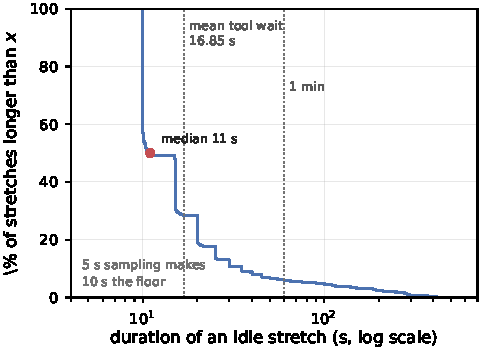
\includegraphics[width=\columnwidth]{figs/fig4_idle_segments.pdf}
  \caption{Survival function of idle-stretch duration, pooled over all
  completed runs (1{,}849 stretches). The median stretch is 11\,s and 30\%
  exceed 20\,s---the same scale as the 16.85\,s mean tool wait, and far above
  the 2\,s control cycle. The vertical cliff at 10\,s is the sampling floor.}
  \label{fig:idle}
\end{figure}

\subsection{Why idle time exists, and why it cannot be recovered}

Idle time is a property of the workload, not of the controller. A session in a
tool wait holds its permit and its KV but issues no request; with only about
two live sessions, the probability that all of them are simultaneously waiting
is substantial. The direct evidence is the duration of the stretches
themselves: they are of the same order as the tool waits, and an order of
magnitude longer than the 2\,s control cycle (Fig.~\ref{fig:idle}). A
controller cannot be blamed for a gap that is set by the tool.

We note one claim we had to drop here. An earlier draft reported that idle
fraction falls monotonically with mean concurrency. With the full data it does
not: \texttt{F:hz0} at 1.41 running requests idles 15.2\% while \texttt{cap4}
at 1.48 idles 10.4\%. The weaker statement that survives is the one we use---%
the stretches are structural and long.

The obvious remedy---keep more sessions live so that someone is always
ready---is what \texttt{bres} does, and it fails for the reason given above.
The structural remedy would be to make the engine do work during a wait, but
there is no work to do: the session's next round does not exist until its tool
returns.
